%!TEX root = ../thesis.tex
\section{Evaluation}

\begin{figure}[t]
  \centering
  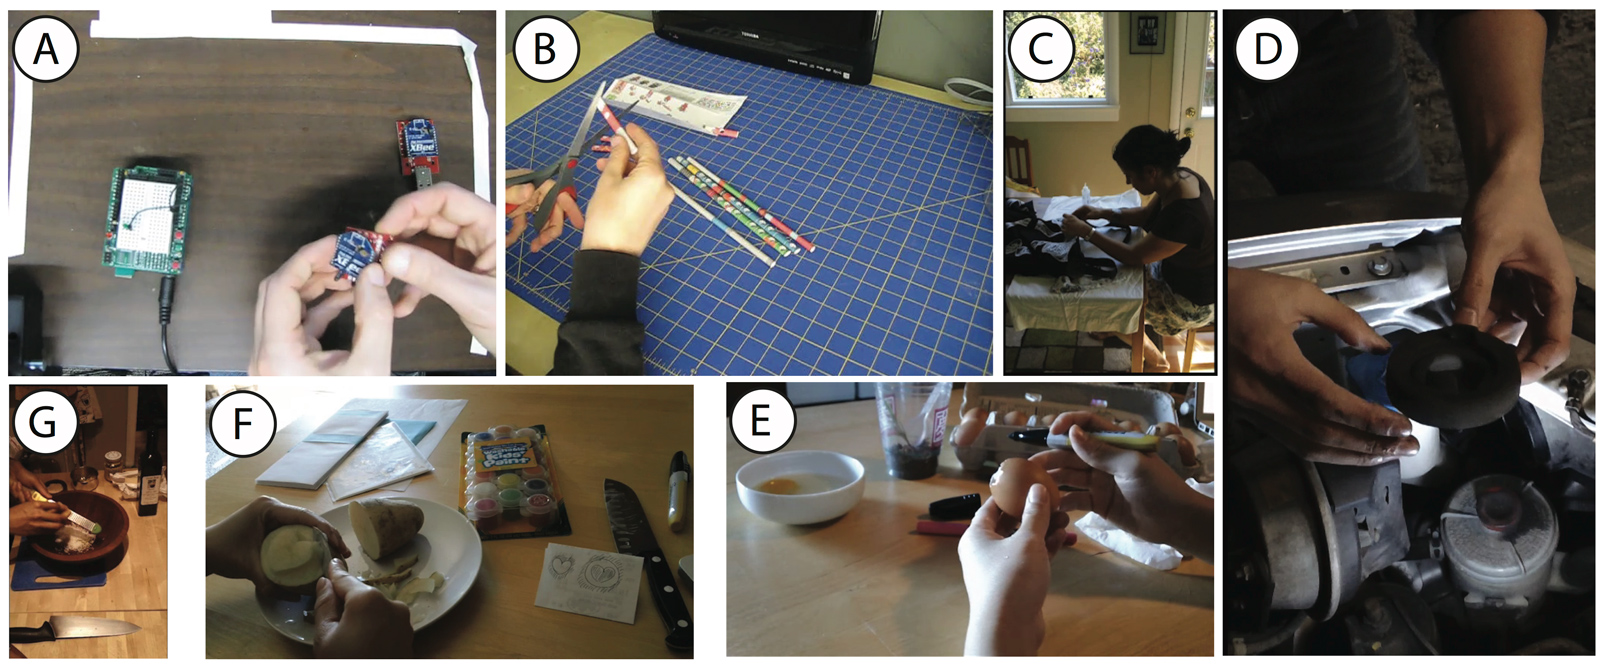
\includegraphics[width=\columnwidth]{\democut/fig/results-small}
  \caption{Illustrative frames from the seven videos used to assess DemoCut. Labels correspond to task labels in Table~\ref{tab:system_results}.}
  \label{fig:results}
  \vspace{-0.2in}
\end{figure}

\subsection{Evaluating Automatic Effect Decision}

To evaluate DemoCut's analysis engine, we recorded seven how-to tasks
from the five categories we selected in the formative user study
(Table~\ref{tab:system_results}).
%
The tasks were recorded by 4 people (all authors of this
work) in 7 locations using a Sony camcorder or an iPad with
a video resolution of at least 640x480 pixels.
%
We used DemoCut to annotate the recordings and then examined the
automatically generated tutorials.

Overall, the resulting tutorials exhibit many of the desired
characteristics outlined earlier in the chapter.
%
The automatically edited videos are concise: 2-5 minutes long and 2.5
times shorter than the original footage.
%
In most cases, DemoCut successfully identified segments where the ``Fast
Motion'' or ``Skip'' effects could be applied to condense the tutorial.
%
For example, the edited salad dressing video uses ``Fast Motion'' to
speed up repetitive actions like chopping an onion and grating cheese,
and then skips the segment where the author leaves the frame to toast
pine nuts.
%
In addition, the automatically generated titles improve the clarity of
the tutorials by adding valuable descriptions of steps, actions,
supplies and indicating the elapsed time for skipped segments.
%
In an electronics tutorial, titles like ``sending data toggles LED''
add important details that are not visible in the video.

There were some situations where the effects were not as successful.
%
To get a more quantitative measure of DemoCut's performance, we
counted several types of errors in the automatically generated
videos:

{\em Incorrect editing effects.} In a few cases, the ``Fast Motion''
effect is applied to segments where the audio track should actually be
in sync with the visuals. Also, when markers are very close to one
another in time, DemoCut sometimes generates very short segments where the editing effects are hard to see.
%
We identify these cases as incorrect editing effects.

{\em Audio miss.} We refer to any piece of narration that is not
detected as a non-silent section as a miss.

{\em Audio cut-off.} We refer to any detected non-silent section that
cuts off narration by ending too early or starting too late as a
cut-off error.

{\em Audio false-positive.} We refer to any non-silent section that is
neither narration nor significant activity or background sound as a false-positive.

We report the incorrect edits as a percentage of the total number of
segments and the three audio errors as a percentage of the total
number of ground-truth narration sections.
%
Table~\ref{tab:system_results} shows all of the results from our
analysis.
%
Overall, we found low average error rates (less than 11\%) for all of
these problems.
%
Also, note that most of these errors can be fixed by changing the
automatically applied editing effects in DemoCut's reviewing and
editing interface.

